\documentclass[11pt]{article}
\usepackage[margin=1in]{geometry}
\usepackage{amsmath,amssymb}
\usepackage{graphicx}
\usepackage{booktabs}
\usepackage{enumitem}
\usepackage[colorlinks=true,linkcolor=black,urlcolor=blue]{hyperref}
\usepackage{titlesec}
\usepackage{parskip}

\titleformat{\section}{\normalfont\large\bfseries}{\thesection}{0.6em}{}
\titleformat{\subsection}{\normalfont\normalsize\bfseries}{\thesubsection}{0.6em}{}

\newcommand{\mhat}{\widehat{m}}
\newcommand{\SD}{\operatorname{SD}}

\title{\vspace{-2em}\bfseries What phase-locked template subtraction does to the\\
heartbeat-evoked potential, and what a QRS-limited template costs}
\author{Companion note to the CFA ear-EEG paper}
\date{\today}

\begin{document}
\maketitle
\vspace{-1.5em}

\noindent
\textbf{Summary.} A cardiac-artifact template indexed by heartbeat phase cannot distinguish the
artifact from a cortical response that is itself phase-locked to the heartbeat. The
heartbeat-evoked potential (HEP) is such a response, and it is reported at roughly $200$--$600$~ms
after the R-peak---inside the template. This is not a risk to be hedged; it is a certainty, and the
only useful question is how much is at stake. This note measures it on the same behind-the-ear
recordings used in the paper, and quantifies the alternative: restricting the template's support to
the QRS interval, which leaves the HEP interval untouched at a measured cost in artifact
suppression.

\section{The identifiability statement}

Write the measurement as $y = s_a + s_p + d_r + n$, splitting the neural signal into a
cardiac-asynchronous part $s_a$ and a part $s_p$ that is phase-locked to the cardiac cycle. The
paper's estimator observes only $y$ and the R-peak instants $\{t_k\}$, and returns a template
$\mhat(\phi)$ that is a function of cardiac phase alone. Both $d_r$ and $s_p$ are functions of
$\phi$ alone. They are therefore \emph{not identifiable} from $(y,\{t_k\})$: no learning rule, gain
schedule, or amount of data separates them, because they are the same object as far as the
observation model is concerned.

Two consequences follow, and they should be stated together rather than traded against each other.
Any phase-locked cortical activity is removed along with the artifact. And a method that avoided
removing it would, by the same argument, have to leave the phase-locked part of the artifact behind.
Separating the two requires information the timing-only estimator does not have---a second channel
with a different mixing, a stimulus-locked contrast, or a model of one of the two components.

\section{Measurement}

We use the two-channel behind-the-ear EEG of SeizeIT2 (OpenNeuro \texttt{ds005873}), high-pass
filtered at $0.5$~Hz, notch filtered at $50$~Hz, resampled onto the ECG grid, with only
supervisor-approved learnable beats entering the average. The analysis window $[-50,600]$~ms
relative to the R-peak is split into a \emph{QRS part} $[-50,200)$~ms and an \emph{HEP part}
$[200,600)$~ms, which partition it exactly, so the energy share attributed to each is a genuine
share.

Since the true disturbance is unobservable on real recordings, the phase-locked content of each
interval is measured against a null that shares the record's statistics but destroys phase locking.
Let $\mathcal{E}_P[z]$ be the energy of the $P$-triggered average of $z$ over the interval of
interest. Averaging on the true peaks gives $\mhat = m + \ell$ with leakage $\ell$ of scale
$\SD/\sqrt{N_r}$; a circular time-shift of the whole peak train preserves the RR-interval sequence
but destroys absolute phase, so it yields leakage only. Averaging $200$ such shifts gives the null
floor $\overline{\mathcal{E}_{\mathrm{scr}}}$, and
\begin{equation}
\mathrm{SNR}_{\mathrm{tmpl}} = 10\log_{10}\frac{\mathcal{E}_{\mathrm{true}}}
{\overline{\mathcal{E}_{\mathrm{scr}}}}
\label{eq:snr}
\end{equation}
is bias-free, the same leakage entering numerator and denominator. Subtracting the floor from
$\mathcal{E}_{\mathrm{true}}$ before taking the per-sample root gives a bias-corrected phase-locked
RMS in microvolts, which is the quantity that can be compared against the HEP amplitudes reported in
the literature.

\section{Results}

Figure~\ref{fig:tmpl} shows the template of the showcase record with both intervals marked. Its
bias-corrected phase-locked RMS is 10.9~$\mu$V over the QRS part and 2.62~$\mu$V over
the HEP part, the latter 16.0~dB above the null ($p<0.01$, $200$ shifts). Across the
84 recordings with a resolvable template (of 436 analyzed; gate
$\mathrm{SNR}_{\mathrm{tmpl}}\ge 10$~dB over the full window) the HEP-interval component is
significant in 80, with median 10.0~dB in that interval alone, median
1.50~$\mu$V and maximum 7.71~$\mu$V RMS. It carries a median 28\% of
the removable phase-locked energy, and the spread is wide: the showcase record is at the favorable
end, with only 8\% of its removable energy past $200$~ms, while at the other extreme a
record's phase-locked energy lies almost entirely there. The showcase should therefore be read as an
illustration of the geometry, not as a typical cost.

\begin{figure}[!ht]
\centering
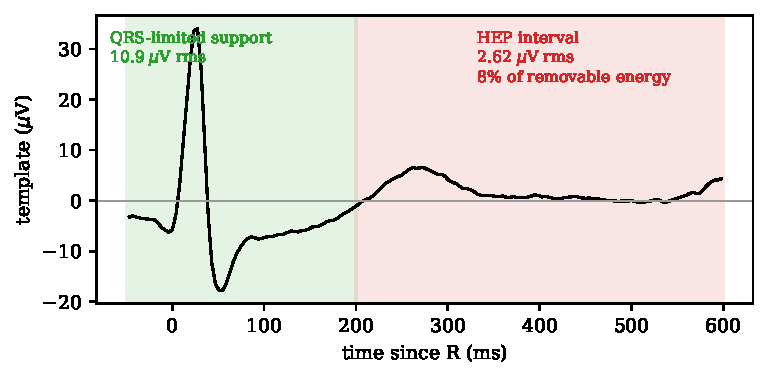
\includegraphics[width=0.72\linewidth]{fig_real/fig_hep_template.pdf}
\caption{Non-causal template of the showcase record (\texttt{ds005873}, sub-070, ses-01, run-20,
behind-the-ear channel, $N_r = 851$ learnable beats of a $600$~s window) against time since the
R-peak. Green: the QRS part $[-50,200)$~ms retained by the QRS-limited template. Red: the HEP part
$[200,600)$~ms, annotated with its bias-corrected phase-locked RMS and its share of the removable
phase-locked energy.}
\label{fig:tmpl}
\end{figure}

Both readings of these numbers matter, and neither on its own settles the question. Read as
artifact, a phase-locked deflection of median 1.50~$\mu$V, reaching 7.71~$\mu$V,
is worth removing, and is of the same order as reported HEP amplitudes---so leaving it in a
continuous recording is not self-evidently safer than removing it. Read as neural signal, that same order of magnitude is exactly why the method must not
be applied unexamined in an HEP study: whatever cortical response occupies the interval is inside
the subtracted template and is not recoverable from it.

\section{The QRS-limited template}

Because the paper's template is defined on the full cardiac cycle rather than on a fixed epoch, a
restricted support costs nothing structurally: set $\mhat(j) = 0$ for every phase bin outside
$[-50,200)$~ms. The HEP interval is then returned to the output identical to the input.

The price is the phase-locked energy in that interval---a median 28\% across the
resolvable recordings, 8\% on the showcase record, and on a minority of records nearly
all of it. The main lobe used for the paper's
$\mathrm{SNR}_{\mathrm{tmpl}}$ figures ($50$~ms pre to $150$~ms post) lies entirely inside the
retained support, so the QRS-limited template accounts for that figure in full.

\section{Recommendation}

\begin{itemize}[leftmargin=1.4em,itemsep=0.2em]
\item \textbf{QRS-limited by default} whenever the downstream analysis is not known in advance, or
whenever heartbeat-locked cortical activity might be examined later. It removes the bulk of the
artifact and forecloses nothing.
\item \textbf{Full-window template} when heartbeat-correlated activity is unambiguously nuisance
contamination---continuous wearable monitoring, decoding of non-cardiac rhythms---and the
$200$--$600$~ms interval will not be interpreted.
\item \textbf{Neither} in a study whose dependent measure is the HEP. The estimator is not
mis-specified there; it is being asked for something no timing-only method can provide.
\end{itemize}

\section*{Reproducing these numbers}

\begin{verbatim}
python src/phase_hep_analysis.py --scan --max-runs 2 --duration-sec 600 \
       --out outputs/phase_hep_scan_full.json
python src/rerun_gated.py --out outputs/phase_hep_gated.json
python src/hep_figure.py --gated outputs/phase_hep_gated.json \
       --out paper/fig_real/fig_hep_template.pdf
\end{verbatim}

\end{document}
